\documentclass{article}

\usepackage{shyne}

% document format
\topmargin 0in
\oddsidemargin 0in
\evensidemargin 0in
\headheight 0in
\headsep 0in
\topskip 0in
\textheight 9in
\textwidth 6.5in
\linespread{1.3}

\begin{document}

\begin{flushleft}
\section*{Group Work - Week 5}

\paragraph{1} The file ``\verb+heights.csv+" on D2L has heights in inches of a sample of 25 men and 25 women.\\ \medskip


\begin{enumalpha}
\item Create 5 number summaries and boxplots for both men and women.\\
\medskip
\bt{5-number summary for men: 62.2, 66.2, 70.3, 74.5, 79.6}\\
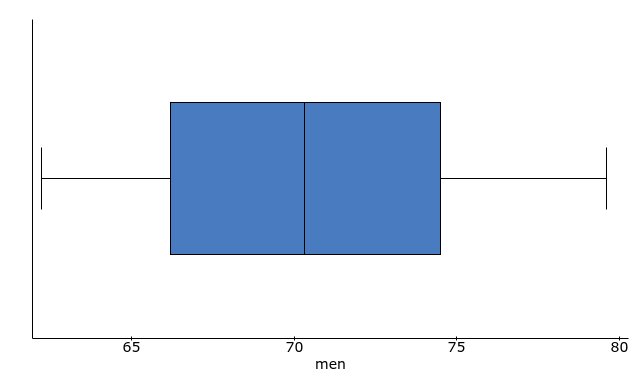
\includegraphics[width=4in]{images/group05_Q1_a_men}\\
\medskip
\bt{5-number summary for men: 54, 59.8, 63.7, 66.8, 71.6}\\
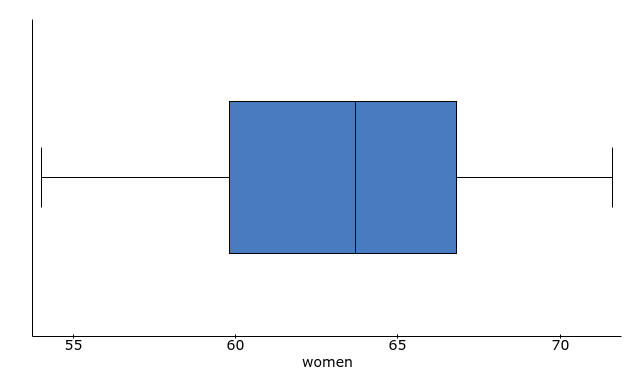
\includegraphics[width=4in]{images/group05_Q1_a_women}\\

\newpage
\item Consider a man who is 68.5 inches tall and a woman who is 63.25 inches tall. What are the z-scores for height for both of these individuals? Who is taller relative to their gender?\\
\medskip
$\ds \bv{\mu_{men} = 	70.236, \qquad \sigma_{men} = 5.037}$\\ \medskip
$\ds \bv{z_{men} = \frac{x - \mu_{men}}{\sigma_{men}} = \frac{68.5 -70.236}{5.037} = -0.347 }$\\
\bigskip
$\ds \bv{\mu_{women} = 	63.292, \qquad \sigma_{women} = 5.280}$\\ \medskip
$\ds \bv{z_{women} = \frac{x - \mu_{women}}{\sigma_{women}} = \frac{63.25 -63.292}{5.280} = -0.008 }$\\
\bigskip
\bt{The woman is taller for her gender.}
\vspace{1in}

\item What percentile is 71 inches for a man? What height is the 80th percentile for women?\\
\medskip
\bt{After sorting the heights of men, 71 is in row 15. Thus, there are 14 values less than 71 and $\bv n$ = 25. Then,}\\ \smallskip
\bt{$\ds \bv{\text{\%ile} =\frac {14}{25} \times 100 = 56 \text{ \%ile}}$}\\
\bigskip



\bt{From StatCrunch, the 80\%ile for women is 69.05.}
\end{enumalpha}

\newpage
\paragraph{2} Suppose you encounter the following game at a school carnival: A wheel with colored spokes is spun and the wheel comes to rest with a pointer pointing at one of the spokes. If you land on a gold spoke, you get 10 tickets. You get 4 tickets for landing on blue and 2 tickets for landing on red. If you land on black, you get nothing. There are 9 black spokes, 6 red spokes, 4 blue and 1 gold spoke. The game cost three tickets to play.

\begin{enumalpha}
\item Create a probability distribution which describes this game.\\
\medskip
{\centering \bt{
\begin{tabular}{c|c}
Tickets won & Probability\\
\hline
0 & $\bv{\frac{9}{20} = 0.45}$\\
2 & $\bv{\frac{6}{20} = 0.3}$\\
4 & $\bv{\frac{4}{20} = 0.2}$\\
10 & $\bv{\frac{1}{20} = 0.05}$\\
\end{tabular}
} \par}
\vspace{0.5in}

\item How many tickets should you expect to win? That is, what is the expected value of the game? What is the standard deviation of tickets won? If you play this game many times, are you likely to end up with more or less tickets than when you started?\\
\medskip
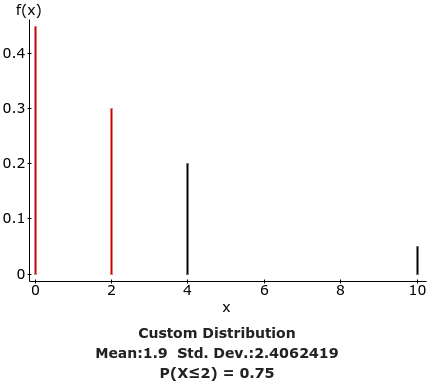
\includegraphics[width=3in]{images/group05_Q2_b}\\ 
\medskip
$\ds \bv{E(X) = \mu = 1.9, \qquad \sigma= 2.4}$\\
\medskip
\bt{On average, you can expect to win 1.9 tickets after spending 3 tickets. Over time you likely lose tickets.}
\vspace{.5in}

\item Is winning 4 tickets a significantly high number of tickets to win?\\
\medskip
$\bv{P(X \ge 4) = 0.25}$\qquad \bt{Not significantly high.}
\end{enumalpha} 
\end{flushleft}
\end{document}